\documentclass[]{slides}
\title{Instruction Set Architecture}

% Begin document
\begin{document}
\printpdftrue % uncomment to hide pauses
% Title slide
\begin{frame} \titlepage \end{frame}

% Outline slide
%\begin{frame}{Outline} \tableofcontents \end{frame}

% ====================
% ISA definition
% ====================
\section{\acl{ISA}}
\begin{frame}{\acl{ISA}}{Definition}
\alertblue{\ac{ISA}}
\begin{itemize}
  \item It is an \alertblue{abstract} concept which defines the portion of a computer that is visible to both the programmer and the compiler.
  \item It is part of the link between an application (something a human does such as video recording, playing music, editing a spreadsheet, etc) and the physical layer of the computer, \ie \ac{HW}.
\end{itemize}
\end{frame}

% ====================
% ISA vs uA
% ====================
\subsection{Architecture vs Microarchitecture}
\begin{frame}{\acl{ISA}}{\acs{ISA} vs \acs{uA}}
\begin{itemize}
  \item \ac{ISA} \alertblue{theoretically} describes how a computer executes its programs. 
  \item It describes:
  \begin{itemize}
    \item The fundamental operations, which are simply referred to as \emph{instructions}, that the computer can execute.
    \item How these instructions are executed.
    \item The semantics and rules required for the interaction of the different building blocks of a computer.
  \end{itemize}      
\end{itemize}
\end{frame}

% ====================
% ISA vs uA
% ====================
\begin{frame}{\acl{ISA}}{\acs{ISA} vs \acs{uA}}
\begin{itemize}
  \item Overall, \ac{ISA} provides valuable information to the programmer.
  \begin{itemize}
  	\item Is a computer stack-, accumulator- or register-based?
  	\item Does the computer have memory? Does it have registers?
  	\item How many steps, \ie clock cycles, does it take to execute instructions?
  	\item Where are operands fetched from?
  	\item Where is the result stored?
  	\item How big are data types?
  \end{itemize}
\end{itemize}
\end{frame}


% ====================
% ISA vs uA
% ====================
\begin{frame}{\acl{ISA}}{\acs{ISA} vs \acs{uA}}
\alertblue{\ac{uA}}
\begin{itemize}
  \item \ac{uA} is more closely related to the \alertblue{physical} implementation of a design, \ie, \ac{uA} determines how the \ac{ISA} is implemented in \ac{HW}.
  \begin{itemize}
    \item For example, it describes which building are necessary in order to model a \ac{uP} and how these building blocks are connected with each other. 
  \end{itemize}
\end{itemize}
\end{frame}

% ====================
% ISA vs uA
% ====================
\begin{frame}{\acl{ISA}}{\acs{ISA} vs \acs{uA}}
\begin{itemize}
  \item The same \ac{ISA} may be physically implemented in a variety of \acp{uA}.
  \begin{itemize}
  	\item For example, one \ac{ISA} could be implemented by different \ac{HW} approaches and vendors such as Intel, ARM or AMD, and all three could have different performances.  
  \end{itemize}
  \item A naive adder example: 
  	\begin{itemize}
  	\item \ac{ISA} specifies data width as 64-bits. 
  	\item \ac{uA} defines the adder as ripple-carry, carry-lookahead, carry-save, carry-select, etc.
  	\end{itemize}
  %\item \ac{ISA} and \ac{uA} influence each other.
\end{itemize}
\end{frame}

% ====================
% ISA vs uA
% ====================
\begin{frame}{\acl{ISA}}{\acs{ISA} vs \acs{uA}}
\begin{itemize}
%  \item The abstraction layer provided by \ac{ISA} is not meant to change.
  \item The goal of a processor designer is to evaluate the different trade-offs between \ac{ISA} and \ac{uA} in order to find a Pareto optimal system.
  \begin{itemize}
    \item Power consumption.
	\item Latency - How long does it take to complete a task.
	\item Throughput - How many tasks can be completed in a given time.
	\item Chip area.
  \end{itemize}	 
\end{itemize}
\end{frame}

% ====================
% ISA vs uA
% ====================
\begin{frame}{\acl{ISA}}{Same \ac{ISA}, different \uA - 45~nm technology}
\begin{figure}[!htb]
  \begin{minipage}{0.5\textwidth}
    \centering
    \begin{itemize}
      \item x86 \ac{ISA}.
      \item Quad Core.
      \item 2.6~GHz.
      \item 125~W.
    \end{itemize}
    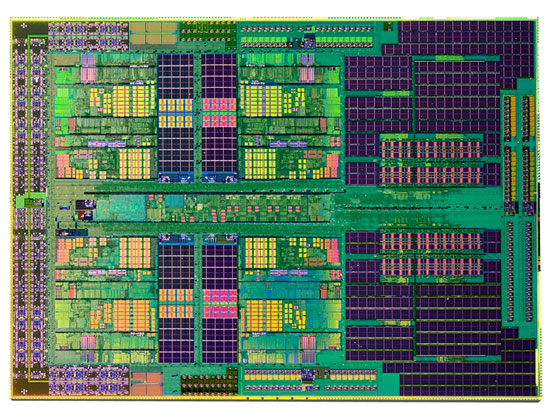
\includegraphics[width=0.8\linewidth]{ISA_AMD_Phenom_II_X4.jpg}
    \caption{AMD Phenom X4}
    \label{Figure:AMD_Phenom_X4a}
  \end{minipage}%
  \begin{minipage}{0.50\textwidth}
    \centering
    \begin{itemize}
      \item x86 \ac{ISA}.
      \item Dual Core.
      \item 1.6~GHz.
      \item 2~W.
    \end{itemize}
    \vspace{14mm}
    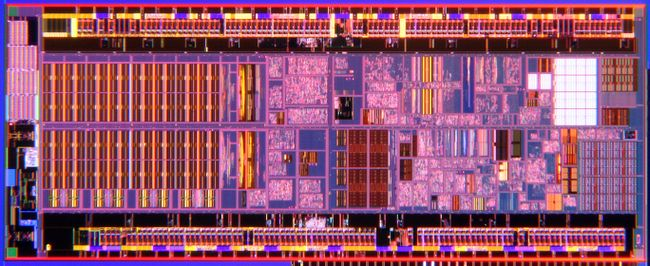
\includegraphics[width=0.92\linewidth]{ISA_Intel_Atom.jpg}
    \caption{Intel Atom}
    \label{Figure:Intel_Atom}
  \end{minipage}
\end{figure}
\end{frame}

% ====================
% ISA vs uA
% ====================
\begin{frame}{\acl{ISA}}{Different \ac{ISA}, different \uA - 45~nm technology}
\begin{figure}[!htb]
  \begin{minipage}{0.5\textwidth}
    \centering
    \begin{itemize}
      \item x86 \ac{ISA}.
      \item Quad Core.
      \item 2.6~GHz.
      \item 125~W.
    \end{itemize}
    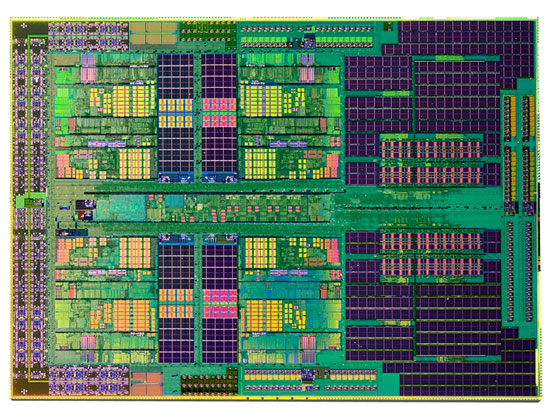
\includegraphics[width=0.8\linewidth]{ISA_AMD_Phenom_II_X4.jpg}
    \caption{AMD Phenom X4}
    \label{Figure:AMD_Phenom_X4b}
  \end{minipage}%
  \begin{minipage}{0.50\textwidth}
    \centering
    \begin{itemize}
      \item Power \ac{ISA}.
      \item Octa Core.
      \item 4.25~GHz.
      \item 200~W.
    \end{itemize}
    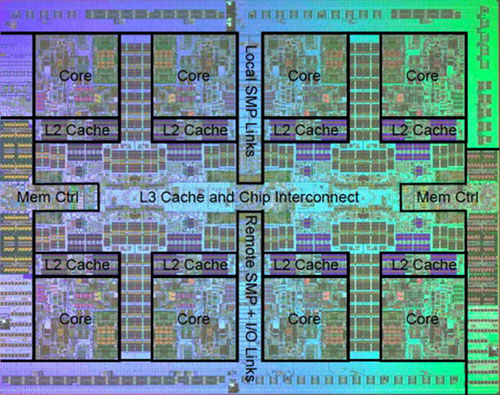
\includegraphics[width=0.75\linewidth]{ISA_IBM_Power7.jpg}
    \caption{IBM Power7}
    \label{Figure:IBM_Power}
  \end{minipage}
\end{figure}
\end{frame}

% ====================
% ISA characteristics
% ====================
\section{\acs{ISA} characteristics}
\begin{frame}{\acs{ISA} characteristics}{}
  \begin{itemize}
    \item Type and size of instructions.
    \item Type and size of operands.
    \item Instruction encoding.
    \item Addressing modes.    
    \item Registers
  \end{itemize}
\end{frame}

% ====================
% ISA characteristics: Registers
% ====================
\section{Registers}
\begin{frame}{\acs{ISA} characteristics}{Registers}
This is list of registers commonly found in \acbf{uP}.
Note that generally, \acp{uP} do not implement every single register in this list.
  \begin{itemize}
    \item \acbf{PC}. Also called \alertblue{IP}, points to the memory address of the next instruction to be executed.
    \item \acbf{RF}. Set of registers used to store data. 
    \item \acbf{SP}. Points to the next location in the stack. Used in \code{PUSH} and \code{POP} operations.
    \end{itemize}
\end{frame}

% ====================
% ISA characteristics: Registers
% ====================
\begin{frame}{Basic registers of a computer}{}
  \begin{itemize}
      \item \acbf{IR}. Holds the instruction currently being executed.
    \item \acbf{MAR}. Also called \acbf{AR}, points to the memory address to/from which data is stored/fetched to/from.
    \item \acbf{IM}. Memory that stores the instructions that the \ac{uP} will execute.
    \end{itemize}
\end{frame}

% ====================
% ISA characteristics: Registers
% ====================
\begin{frame}{Basic registers of a computer}{}
  \begin{itemize}
    \item \acbf{ACC}. Holds the result of arithmetic and logic operations.
    \item \acbf{DM}. Also called \acbf{DR}, holds operand(s) to be used in arithmetic and logic operations.
    \item \acbf{GPR}. Registers to temporary store data or addresses.
    \item \acbf{SR}. Also called \acbf{FR}, holds the special conditions of the result of arithmetic and logic operations, as well as branch and jump status. For example, indicates if a comparison resulted in an equality, if the result of an operation is zero, overflow, etc.
    \end{itemize}
\end{frame}

% ====================
% ISA characteristics: Registers
% ====================
\begin{frame}{Basic registers of a computer}{}
\begin{figure}
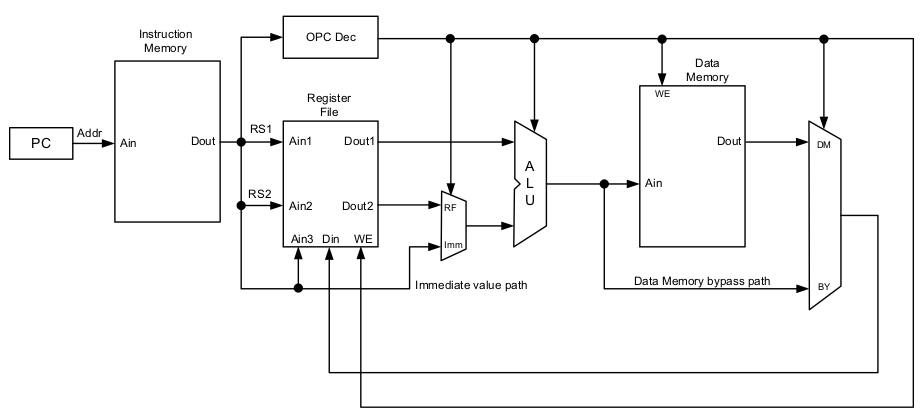
\includegraphics[scale=0.36]{ISA_basic_processor}
\caption{Basic structure of a \ac{uP}.}
\label{Figure:basic_registers}
\end{figure}
\end{frame}

\section{Instructions}
% ====================
% ISA characteristics: Instructions
% ====================
\begin{frame}{\acs{ISA} characteristics}{Instructions}
\begin{itemize}
\item Instructions are the basic operations that a \ac{uP} can understand and perform.
\item The complete set of instructions that a \ac{uP} may perform is called \alertblue{instruction set}, \alertred{which is not the same as \acl{ISA}!}
\end{itemize}
\end{frame}

% ====================
% ISA characteristics: Instructions
% ====================
\begin{frame}{\acs{ISA} characteristics}{Instructions}
\begin{table}[htbp]
    \centering
      \begin{tabular}{l|l}
        \hline
  	    \textbf{Instruction type} & \textbf{Example}\footnote{These examples are not specific to a particular \acs{ISA}.} \\
  	    \hline
  	    \hline
  	    Arithmetic \& logical   & \code{ADD}, \code{SUB}, \code{AND}, \code{OR} \\
  	    \hline
  	    Data transfer           & \code{LOAD}, \code{SW}, \code{MOV}, \code{PUSH}, \code{POP} \\
  	    \hline
  	    Conditional branch      & \code{BNE}, \code{BEQ}  \\
  	    \hline
  	    Unconditional jumps     & \code{JMP}, \code{JAL}, \code{CALL}, \code{RET} \\
  	    \hline
  	    System                  & \code{RD\_INT}, \code{PRNT\_CHR} \\
  	    \hline
  	    Floating Point          & \code{FADD}, \code{FMULT} \\
  	    \hline
  	    %Decimal                 & \code{DADD}, \code{DMULT} \\
  	    %\hline
  	    String                  & \code{MOVSB}, \code{STR\_MV}, \code{STR\_CMP}\\
  	    \hline
  	    Signal processing\footnote{Typically found in \ac{SIMD} \acsp{ISA}.} & \code{ADD\_ARRAY}, \code{MULT\_ARRAY}, \code{FFT}\\
  	    \hline
  	  \end{tabular}
  \end{table}
\end{frame}

% ====================
% ISA characteristics: Instructions
% ====================
\begin{frame}{\acs{ISA} characteristics}{Instructions}
\vspace{-17pt}
\begin{table}[htbp]
    \centering
    \caption{Intel's 80x86 top ten instructions based on five SPECint92 programs\footnote{J. L. Hennessy and D. A. Patterson, \emph{Computer architecture: A quantitative approach}, 6th ed., p A-4, Morgan Kaufmann, 2019.}.}
      \begin{tabular}{r|l|r}
        \hline
  	    \textbf{Rank} & \textbf{Type} & \textbf{Distribution} \\
  	    \hline
  	    \hline
  	    1 & load                        & 22\% \\ \hline
        2 & conditional branch          & 20\% \\ \hline
        3 & compare                     & 16\% \\ \hline
        4 & store                       & 12\% \\ \hline
        5 & add                         & 8\%  \\ \hline
        6 & and                         & 6\%  \\ \hline
        7 & sub                         & 5\%  \\ \hline
        8 & move register-register      & 4\%  \\ \hline
        9 & call                        & 1\%  \\ \hline
       10 & return                      & 1\%  \\ \hline\hline
    \multicolumn{2}{r|}{\textbf{Total}} & \textbf{96\%} \\ \hline
  	  \end{tabular}
  \end{table}
\end{frame}

% ====================
% ISA characteristics: Operands and operations
% ====================
\section{Operands and operations}
\begin{frame}{\acs{ISA} characteristics}{Operands and operations}
	\begin{itemize}
	\item Where do operands come from?
	\item Where are results stored? 
	\item What is the size of the operands?
	\item How many steps does an instruction take?
  \end{itemize}
\end{frame}

% ====================
% ISA characteristics: Operands and operations
% ====================
\begin{frame}{\acs{ISA} characteristics}{Operands and operations}
\begin{figure}[!htb]
    \centering
    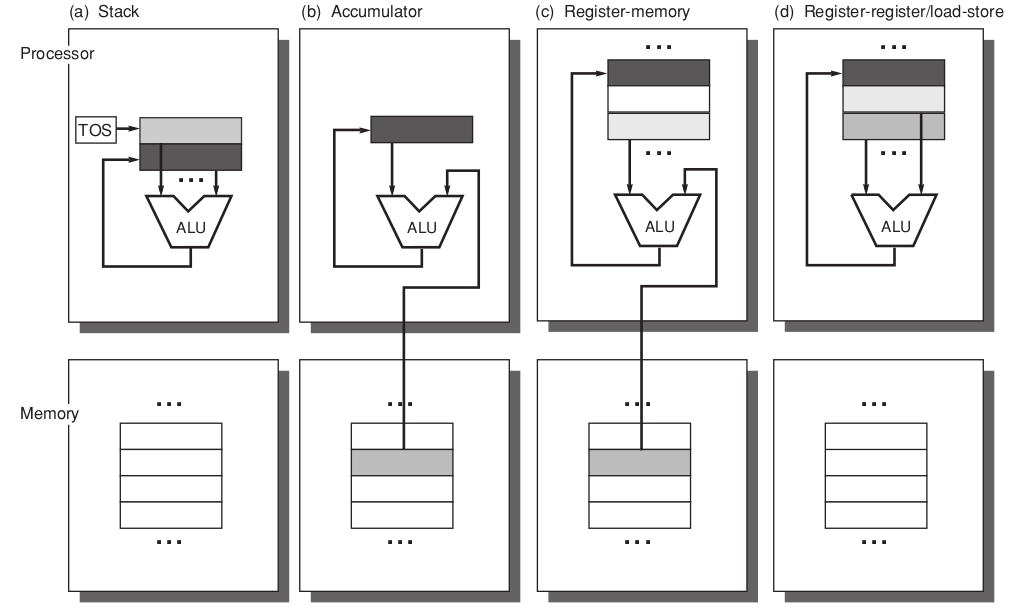
\includegraphics[width=0.75\linewidth]{ISA_Operand_locations.png}
    \caption{Operand locations for different \acp{ISA} [Figure A.1]~\footnote{J. L. Hennessy and D. A. Patterson, \emph{Computer architecture: A quantitative approach}, 6th ed., p A-4, Morgan Kaufmann, 2019.}.}
    \label{Figure:Operand_locations}
\end{figure}
\end{frame}

% ====================
% ISA characteristics: Operands and operations
% ====================
\begin{frame}{\acs{ISA} characteristics}{Operands and operations}
\begin{minipage}{0.5\textwidth}
  \centering        
  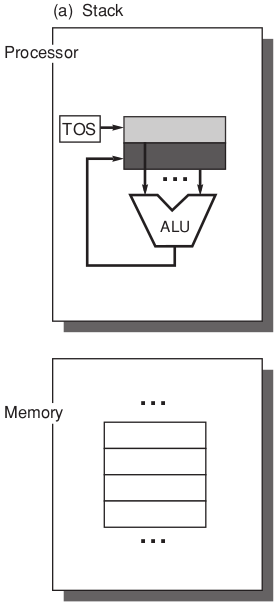
\includegraphics[width=0.55\linewidth]{ISA_Operands_1_Stack.png}
\end{minipage}%
\begin{minipage}{0.50\textwidth}
  \begin{table}[htbp]
    \begin{flushleft}
      \begin{tabular}{ll}
	    \multicolumn{2}{c}{Stack-based \ac{ISA}}\\
		\multicolumn{2}{c}{\code{C = A + B}}\\
		            &          \\
		\code{Push} & \code{A} \\
		\code{Push} & \code{B} \\
		\code{Add}  &          \\
		\code{Pop}  & \code{C}
		\end{tabular}
	\end{flushleft}
  \end{table}
\end{minipage}
\end{frame}

% ====================
% ISA characteristics: Operands and operations
% ====================
\begin{frame}{\acs{ISA} characteristics}{Operands and operations}
\begin{minipage}{0.5\textwidth}
  \centering        
  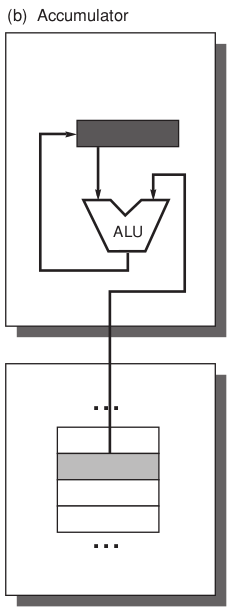
\includegraphics[width=0.45\linewidth]{ISA_Operands_2_Accumulator.png}
\end{minipage}%
\begin{minipage}{0.50\textwidth}
  \begin{table}[htbp]
    \begin{flushleft}
	  \begin{tabular}{ll}
        \multicolumn{2}{c}{Accumulator-based \ac{ISA}} \\
        \multicolumn{2}{c}{\code{C = A + B}}           \\
		             &                                 \\
        \code{Load}  & \code{A}                        \\
		\code{Add}   & \code{B}                        \\
		\code{Store} & \code{C}  
		\end{tabular}
	  \end{flushleft}
	\end{table}
\end{minipage}
\end{frame}

% ====================
% ISA characteristics: Operands and operations
% ====================
\begin{frame}{\acs{ISA} characteristics}{Operands and operations}
\begin{minipage}{0.5\textwidth}
  \centering        
  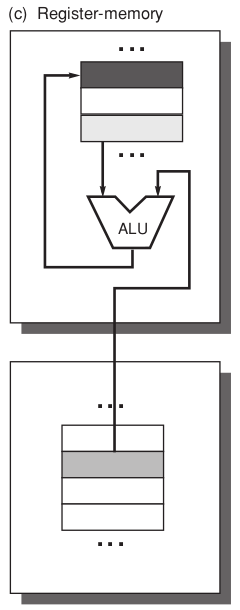
\includegraphics[width=0.45\linewidth]{ISA_Operands_3_Register_Memory.png}
\end{minipage}%
\begin{minipage}{0.50\textwidth}
  \begin{table}[htbp]
    \begin{flushleft}
      \begin{tabular}{llll}
  	    \multicolumn{4}{c}{Memory-Register-based \ac{ISA}}\\
  	    \multicolumn{4}{c}{\code{C = A + B}}              \\
  	                 &                                    \\
  	    \code{Load}  & \code{R1} & \code{A}               \\
  	    \code{Add}   & \code{R3} & \code{R1} & \code{B}   \\
  	    \code{Store} & \code{R3} & \code{C}  
  	  \end{tabular}
    \end{flushleft}
  \end{table}
\end{minipage}
\end{frame}

% ====================
% ISA characteristics: Operands and operations
% ====================
\begin{frame}{\acs{ISA} characteristics}{Operands and operations}
\begin{minipage}{0.5\textwidth}
  \centering        
  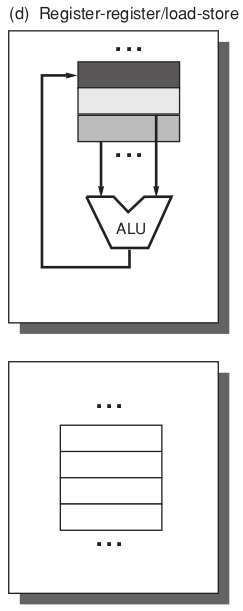
\includegraphics[width=0.45\linewidth]{ISA_Operands_4_Register_Register.png}
\end{minipage}%
\begin{minipage}{0.50\textwidth}
  \begin{table}[htbp]
    \begin{flushleft}
	  \begin{tabular}{llll}
	    \multicolumn{4}{c}{Register-Register-based \ac{ISA}}\\
	    \multicolumn{4}{c}{\code{C = A + B}}                \\
		             &                                      \\
		\code{Load}  & \code{R1} & \code{A}                 \\
		\code{Load}  & \code{R2} & \code{B}                \\
		\code{Add}   & \code{R3} & \code{R1} & \code{R2}      \\  
		\code{Store} & \code{R3} & \code{C}                 \\			
	  \end{tabular}
    \end{flushleft}
  \end{table}
\end{minipage}
\end{frame}

% ====================
% ISA characteristics: Addressing Modes
% ====================
\section{Addressing Modes}
\begin{frame}{\acs{ISA} characteristics}{Addressing modes}
\begin{itemize}
\item How can we read/write data from/into memory?
\item What types of memory exist?
\end{itemize}
\end{frame}

% ====================
% ISA characteristics: Addressing Modes
% ====================
\begin{frame}{\acs{ISA} characteristics}{Addressing modes}
\vspace{-17pt}
\begin{table}[htbp]
    \centering
    \caption{Examples of addressing modes}
      \begin{tabular}{l|l|l}
       \AddressModesHeader
       \Immediate
       \Register
       \Absolute
       \RegisterIndirect
       \Indexed
       \Displacement
       \MemoryIndirect
       \hline
  	  \end{tabular}
  \end{table}
\end{frame}

% ====================
% ISA characteristics: Addressing Modes
% ====================
\begin{frame}{\acs{ISA} characteristics}{Addressing modes}
\vspace{-17pt}
\begin{table}[htbp]
    \centering
    \caption{Examples of addressing modes}
      \begin{tabular}{l|l|l}
       \AddressModesHeader
       \Autoincrement
       \Autodecrement
       \Scaled
       \hline
  	  \end{tabular}
  \end{table}
  \textbf{Note} that Autoincrement and Autodecrement modes, the order of + and - signs influence the order of the operations. 
  For example, \code{-(R2)} indicates decrementing \code{R2} before accessing to memory.
\end{frame}

% ====================
% ISA characteristics: Addressing Modes
% ====================
\subsection{Addressing Modes: Examples}
\begin{frame}{\acs{ISA} characteristics}{Addressing modes: Example}
  \begin{itemize}
    \item Let's assume that registers \code{Ri}, $i\in [1,4]$, and selected memory locations of a computer store the following values. 
  \end{itemize}
\begin{minipage}{0.25\textwidth}
\vspace{-44pt}
  \begin{table}[htbp]
    \begin{tabular}{r|r}
	  \textbf{Reg} & \textbf{Val}\\ \hline\hline
	  \R1 & 23 \\ \hline
	  \R2 & 11 \\ \hline
	  \R3 &  7 \\ \hline
	  \R4 & 19 \\ \hline
    \end{tabular}
  \end{table}
\end{minipage}%
\begin{minipage}{0.25\textwidth}
  \begin{flushleft}
    \begin{table}[htbp]
      \begin{tabular}{r|r}
	    \textbf{Mem} & \textbf{Val}\\ \hline\hline
	     7 & 23 \\ \hline
	    11 & 13 \\ \hline
	    13 & 31 \\ \hline
	    23 & 17 \\ \hline
	    34 & 37 \\ \hline
	   100 & 13 \\ \hline
	   123 & 29 \\ \hline
	   132 & 41 \\ \hline
      \end{tabular}
    \end{table}
  \end{flushleft}
\end{minipage} 
\end{frame}

% ====================
% ISA characteristics: Addressing Modes
% ====================
\AddrModeEx{\Immediate}{\R4}{}
\AddrModeEx{\Register}{\R4}{}
\AddrModeEx{\Absolute}{\R2}{}
\AddrModeEx{\RegisterIndirect}{\R4}{}
\AddrModeEx{\Indexed}{\R3}{}
\AddrModeEx{\Displacement}{\R4}{}
\AddrModeEx{\MemoryIndirect}{\R1}{}
\AddrModeEx{\Autoincrement}{\R1}{3}
\AddrModeEx{\Autodecrement}{\R1}{4}
\AddrModeEx{\Scaled}{\R1}{3}

% ====================
% ISA characteristics: Instruction encoding
% ====================
% http://inst.eecs.berkeley.edu/~cs61c/resources/su18_lec/
\section{Instruction encoding}
\begin{frame}{\acs{ISA} characteristics}{Instructions encoding}
  \begin{itemize}
      \item In stored-program computers, instructions and data are stored in memory.
    \item So, how does a processor know
    \begin{itemize}
        \item how to differentiate between operations and operands?
    	\item which instruction to perform?
    	\item which \code{Reg} or \code{Mem} locations are the operands located?
        \item which \code{Reg} or \code{Mem} locations should the result be stored to?
        \pauseprint
        \item how to differentiate between
	\end{itemize}
	~~~~~~\code{\R1 $\leftarrow$ \R2 + \R3}\\
	~~~~~~\code{\R1 $\leftarrow$ \R2 + \Mem{R3}}\\
	~~~~~~\code{\R1 $\leftarrow$ \R2 + \Mem{\Mem{R3}}}\\
	~~~~~~\code{\R1 $\leftarrow$ \Mem{R2} + \Mem{R3}}\\
      \item Instruction encoding is a \alertblue{convention used to differentiate the various operations in a \ac{uP}, as well as operations from operands}.
  \end{itemize}
\end{frame}

% ====================
% ISA characteristics: Instruction encoding
% ====================
\begin{frame}{\acs{ISA} characteristics}{Instructions encoding}
  \begin{itemize}	
    \item Instructions are encoded using binary representation.
\item Suppose we want to design a processor that can implement the following instructions.\\
    ~~~~~~\code{\R1 $\leftarrow$ \R2 + \R3}\\
	~~~~~~\code{\R1 $\leftarrow$ \R2 + \Mem{R3}}\\
	~~~~~~\code{\R1 $\leftarrow$ \R2 + \Mem{\Mem{R3}}}\\
	~~~~~~\code{\R1 $\leftarrow$ \Mem{R2} + \Mem{R3}}\\\pauseprint
    \item We could assign a binary code to each of these 4 operations.
  \end{itemize}
    \begin{table}[htbp]
      \centering
        \begin{tabular}{l|l}
          \hline
          \textbf{Instruction} & \textbf{Binary code}\\
          \hline\hline
          \code{\R1 $\leftarrow$ \R2 + \R3}            & 00 \\ \hline
          \code{\R1 $\leftarrow$ \R2 + \Mem{R3}}       & 01 \\ \hline
          \code{\R1 $\leftarrow$ \R2 + \Mem{\Mem{R3}}} & 10 \\ \hline
          \code{\R1 $\leftarrow$ \Mem{R2} + \Mem{R3}}  & 11 \\ \hline
  	    \end{tabular}
    \end{table}
    \pauseprint
  \begin{itemize}
    \item Let's try to expand this implementation.
  \end{itemize}
\end{frame}

% ====================
% ISA characteristics: Instruction encoding
% ====================	
\begin{frame}{\acs{ISA} characteristics}{Instructions encoding: A naive example}
  \begin{itemize}
    \item Let \Rd be the destination register and \Rs{i} the source register, where $\mathtt{d} \in [0,3]$ and $\mathtt{i} \in [0,3]$.
    \item We could assign a binary code for each combination of \Rd and \Rs{i} in the instruction \Rd $\leftarrow$ \Rs{1} + \Rs{2}.
    \pauseprint
  \end{itemize} 
  \vspace{-3pt}
  \begin{table}[htbp]
    \centering
    \begin{tabular}{c|c|c}
      \hline
      \textbf{Instruction} & \textbf{Binary code} & \textbf{Hex code}\\
      \hline\hline
      \code{\R0 $\leftarrow$ \R0 + \R0} & 00 0000 & \hex{00} \\ \hline
      \code{\R0 $\leftarrow$ \R0 + \R1} & 00 0001 & \hex{01} \\ \hline
      \vdots                            & \vdots & \vdots  \\ \hline
      \code{\R1 $\leftarrow$ \R2 + \R3} & 01 1011 & \hex{1B} \\ \hline
      \vdots                            & \vdots & \vdots  \\ \hline
      \code{\R2 $\leftarrow$ \R3 + \R0} & 10 1100 & \hex{2C} \\ \hline
      \vdots                            & \vdots & \vdots  \\ \hline
      \code{\R3 $\leftarrow$ \R3 + \R3} & 11 1111 & \hex{3F} \\ \hline
  	\end{tabular}
  \end{table}
\end{frame}

% ====================
% ISA characteristics: Instruction encoding
% ====================	
\begin{frame}{\acs{ISA} characteristics}{Instructions encoding: A naive example} 
  \begin{itemize}
    \item What about the \uA~of this encoding?
  \end{itemize}
  \pauseprint
\begin{figure}[!htb]
  \centering
  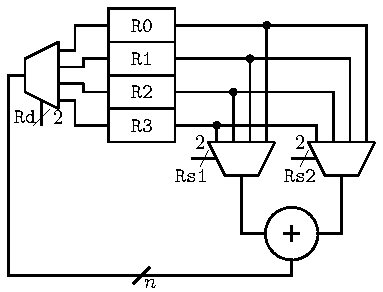
\includegraphics[width=0.57\linewidth]{ISA_naive_uA_example}
  \caption{A naive \uA~for adding two registers.}
  \label{Figure:NaiveuA}
\end{figure}
\end{frame}

% ====================
% ISA characteristics: Instruction encoding
% ====================
\begin{frame}{\acs{ISA} characteristics}{Instructions encoding}
  \begin{itemize}
    \item Is our previous scheme feasible?
    \item What's wrong with it?
	\item Could it be generalised?   
    \item What about other addressing modes?  
    \item How could we include other operations such as subtractions or jumps?
    \item Are all instructions represented using the same number of bits?
  \end{itemize}     
\end{frame}

% ====================
% ISA characteristics: Instruction encoding
% ====================	
\begin{frame}{\acs{ISA} characteristics}{Instructions encoding}
\begin{itemize}
\item We can continue to expand this scheme in order to add other operations, \eg, subtraction and logical operations.
\item Moreover, we can continue to include bits that represent different addressing modes.
\item The ultimate goal of this, is to design an encoding feasible for all operations and addressing modes in our \ac{ISA}.
\end{itemize} 
\end{frame}

% ====================
% ISA characteristics: Instruction encoding
% ====================
\begin{frame}{\acs{ISA} characteristics}{Instructions encoding}
\vspace{-5pt}
  \begin{itemize}
    \item \small{We could have a bit for selecting addition/subtraction in our previous design.}
    \pauseprint
  \end{itemize} 
  \vspace{-3pt}
  \begin{table}[htbp]
    \centering
    \vspace{-10pt}
    \caption{Naive encoding for adding and subtracting two numbers.}
  	\label{Table:Naive_encoding}
  	\vspace{-5pt}
    \begin{tabular}{c|c|c}
      \hline
      \textbf{Instruction} & \textbf{Binary code} & \textbf{Hex code}\\
      \hline\hline
      \code{\R0 $\leftarrow$ \R0 + \R0} & \alertblue{0}00 0000  & \hex{00} \\ \hline
      \vdots                            & \vdots & \vdots  \\ \hline
      \code{\R1 $\leftarrow$ \R2 + \R3} & \alertblue{0}01 1011  & \hex{1B} \\ \hline
      \vdots                            & \vdots & \vdots  \\ \hline
      \code{\R3 $\leftarrow$ \R3 + \R3} & \alertblue{0}11 1111  & \hex{3F} \\ \hline
            \code{\R0 $\leftarrow$ \R0 - \R0} & \alertblue{1}00 0000  & \hex{10} \\ \hline
      \vdots                            & \vdots & \vdots  \\ \hline
      \code{\R1 $\leftarrow$ \R2 - \R3} & \alertblue{1}01 1011  & \hex{5B} \\ \hline
      \vdots                            & \vdots & \vdots  \\ \hline
      \code{\R3 $\leftarrow$ \R3 - \R3} & \alertblue{1}11 1111  & \hex{7F} \\ \hline
  	\end{tabular}
  \end{table}
\end{frame}

% ====================
% ISA characteristics: Instruction encoding
% ====================	
\begin{frame}{\acs{ISA} characteristics}{Instructions encoding}
  \begin{itemize}
	\item As seen in the previous example, the source, destination and operation type may be represented with a \alertblue{single} binary code.
	\item This concept may be further expanded for other operations and addressing modes.
	\item For this purpose, we may use longer binary codes, which may be divided into several fields.
	\item For example, we may use a field called \alertblue{opcode} in order to represent the type of operation to be performed.
	\item Another field may represent the \alertblue{source}, \ie, the memory location where data to operate with is.
	\item Another field may represent the \alertblue{destination}, \ie, the memory location where the result of the operation should be stored to. 
  \end{itemize}     
\end{frame}

% ====================
% ISA characteristics: Instruction encoding
% ====================	
\begin{frame}{\acs{ISA} characteristics}{Instructions encoding}
\vspace{-7pt}
\begin{figure}
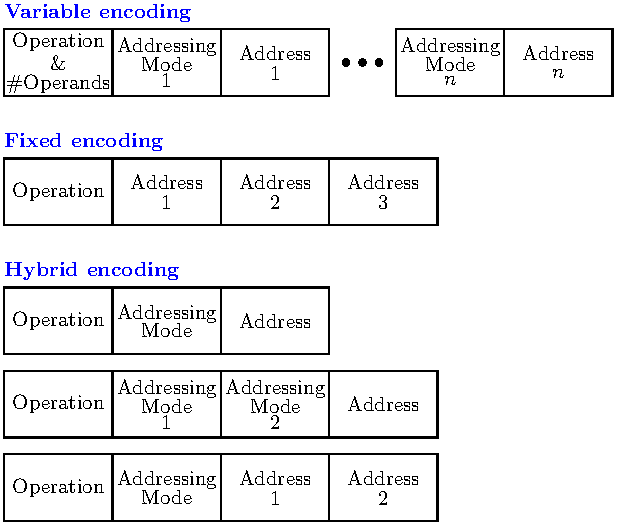
\includegraphics[scale=0.75]{ISA_types_instruction_encoding}
\vspace{-2pt}
\caption{Generalised instruction encoding.}
\label{Figure:types_instruction_encoding}
\end{figure}   
\end{frame}

% ====================
% ISA characteristics: Instruction encoding
% ====================
\begin{frame}{\acs{ISA} characteristics}{Instructions encoding}
\begin{itemize}
  \item \alertblue{Variable encoding.} 
 \begin{itemize}
    \item Supports any number of operands, with each operand having a specific addressing mode.
    \item The number of encoded bits varies between instructions.
    \item \alertdarkgreen{Compact machine programs.}
    \item \alertred{Harder to decode.}
  \end{itemize}
  \item \alertblue{Fixed encoding.} 
  \begin{itemize}
    \item Every instruction has the same number of operands, with addressing modes specified in the opcode.
    \item The number of encoded bits is always the same regardless of the instruction or addressing modes of the operands.
    \item \alertdarkgreen{Easier to decode.}
    \item \alertred{Wasted bits in some instructions.}
  \end{itemize}
  \item \alertblue{Hybrid encoding.}
  \begin{itemize}
  \item Instructions with two different encoding lengths (16- and 32-bits, for example).
  \end{itemize}
\end{itemize}   
\end{frame}

% ====================
% ISA characteristics: Instruction encoding
% ====================	
\begin{frame}{\acs{ISA} characteristics}{Instructions encoding}
  \begin{itemize}
    \item \acp{ISA} may be classified into two main categories according to the complexity of their instruction encoding.
    \item \alertblue{\ac{RISC}.}
    \item \alertblue{\ac{CISC}.}
  \end{itemize}     
\end{frame}

% ====================
% ISA characteristics: CISC encoding
% ====================	
\begin{frame}{\acs{ISA} characteristics}{CISC}
\alertviolet{CISC}
  \begin{itemize}
    \item \acp{ISA} that perform complex operations and the instruction formats are not uniform.
    \item Large number of instructions available.
    \item Microcode approach. 
    \begin{itemize}
      \item A single instruction may be divided into several smaller instructions. 
      \item For example, a single instruction may perform a load from memory, an arithmetic operation and a store to memory.
    \end{itemize}
    \item Reduced size of the compiled code due to \alertviolet{variable-length} encoding. 
    \begin{itemize}
      \item Shortest encodings represent the most commonly used instructions.     
    \end{itemize}

  \end{itemize}    
\end{frame}

% ====================
% ISA characteristics: CISC encoding
% ====================	
\begin{frame}{\acs{ISA} characteristics}{CISC}
\alertorange{RISC}
  \begin{itemize}
    \item \acp{ISA} that have a small number of simple, \alertorange{fixed-length} instructions.
    \item Single-cycle instructions.
    \item Load-store approach. 
    \begin{itemize}
      \item Only load and store instructions are used for transferring data between registers and memory.
    \end{itemize}
  \end{itemize}     
\end{frame}

% ====================
% ISA characteristics: CISC vs RISC
% ====================
\begin{frame}{\acs{ISA} characteristics}{CISC vs RISC}
\vspace{-8pt}
\begin{figure}
\centering
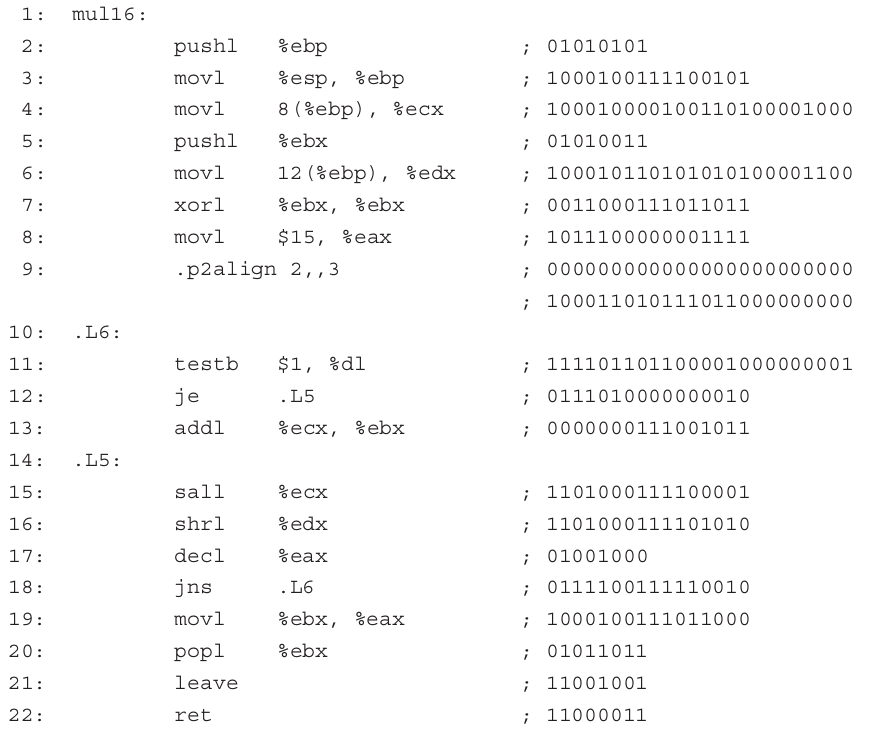
\includegraphics[scale=0.265]{ISA_CISC_code_example}
\vspace{-12pt}
\caption{CISC code example.}
\label{Figure:CISC_code}
\end{figure}    
\end{frame}

% ====================
% ISA characteristics: CISC vs RISC
% ====================	
\begin{frame}{\acs{ISA} characteristics}{CISC vs RISC}
\vspace{-8pt}
\begin{figure}
\centering
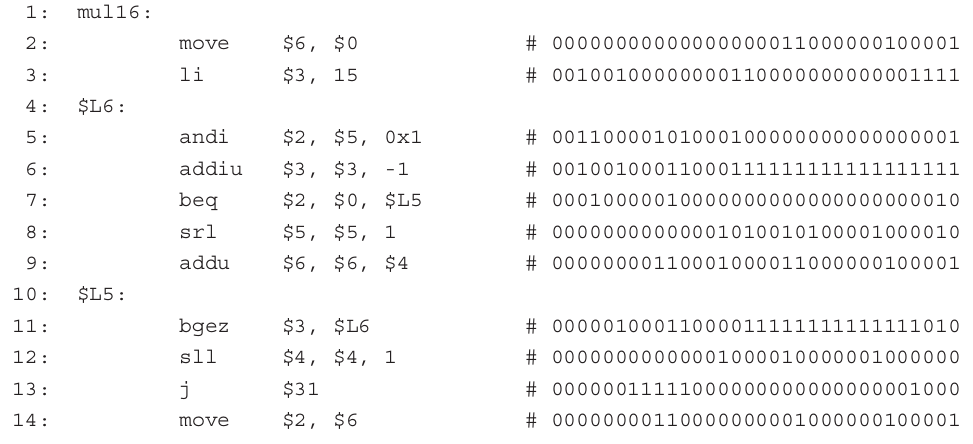
\includegraphics[scale=0.35]{ISA_RISC_code_example}
\vspace{-8pt}
\caption{RISC code example.}
\label{Figure:RISC_code}
\end{figure}    
\end{frame}

% ====================
% ISA characteristics: RISC example
% ====================
\section{RISC-V}	
\begin{frame}{\acs{ISA} characteristics}{RISC-V example}
\textbf{\ac{RISC}-V} main features.
\begin{itemize}
\item 32-bit encoding.
\item 4 types of instructions.
  \begin{itemize}
    \item R-type. Register.
    \item I-type. Immediate.
    \item S-type. Store, compare and branch.
    \item U-type. Jump.
  \end{itemize}
\end{itemize}
\end{frame}

% ====================
% ISA characteristics: RISC example
% ====================	
\begin{frame}{\acs{ISA} characteristics}{RISC-V example}
\vspace{-8pt}
\begin{figure}
\centering
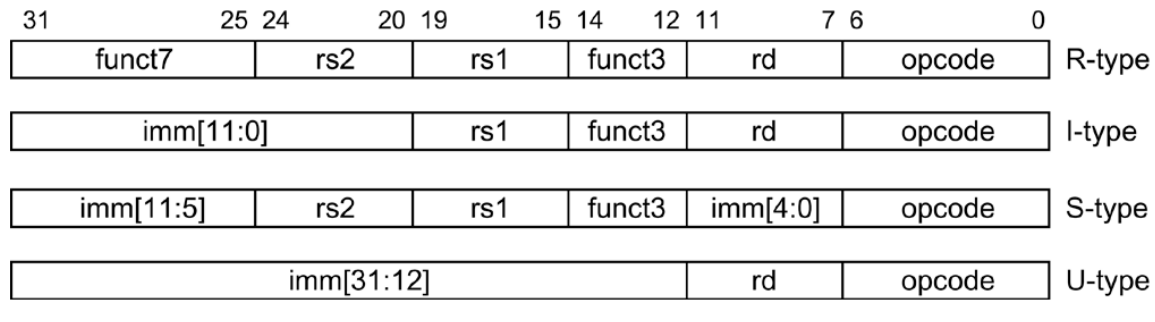
\includegraphics[width=\textwidth]{ISA_RISCV_instruction_types}
\vspace{-8pt}
\caption{RISC instruction format.}
\label{Figure:RISC_instruction_format}
\end{figure}    
\end{frame}

% ====================
% ISA characteristics: RISC example
% ====================
\begin{frame}{\acs{ISA} characteristics}{RISC encoding example}
\begin{itemize}
\item \code{funct7} and \code{funct3} complement the opcode.
\item \code{rd}, \code{rs1} and \code{rs2} are destination, source 1 and source 2 registers, respectively.
\item \code{imm} is an immediate value.
\end{itemize}
\end{frame}

% ====================
% ISA characteristics: RISC example
% ====================	
\begin{frame}{\acs{ISA} characteristics}{RISC encoding example}
\vspace{-8pt}
\begin{figure}
\centering
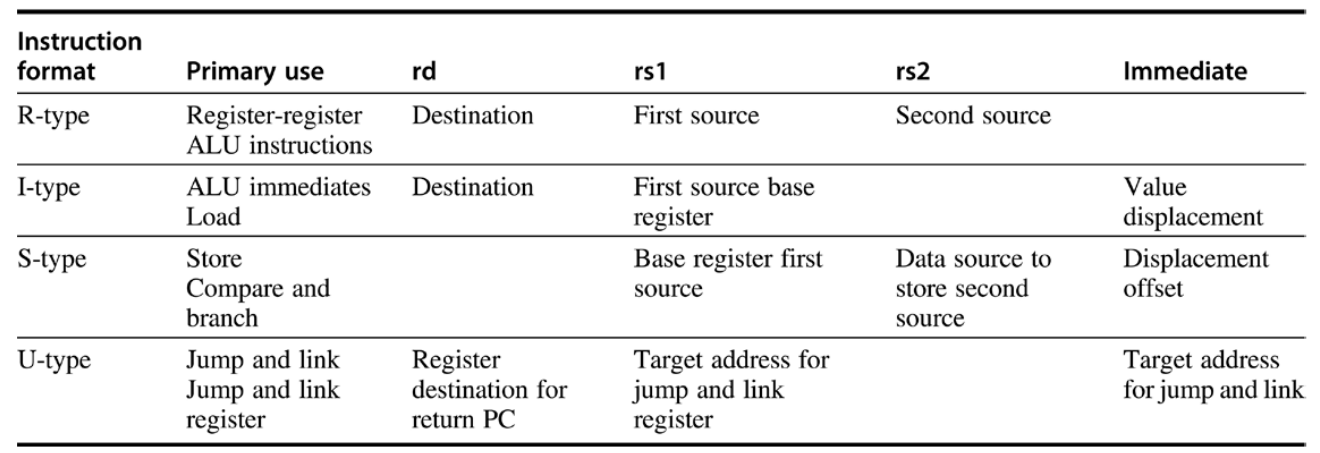
\includegraphics[width=\textwidth]{ISA_RISCV_instruction_description}
\vspace{-8pt}
\caption{RISC instruction description.}
\label{Figure:RISC_instruction_description}
\end{figure}    
\end{frame}

% ====================
% ISA characteristics: Instructions encoding
% ====================
\begin{frame}{\acs{ISA} characteristics}{Instructions encoding}
  \textbf{\large{QUIZ}} \\
  \begin{itemize}
    \item Which of the following are affected by the instruction encoding?
    \begin{enumerate}
      \item[A)] The execution time of each instruction.
      \item[B)] The \uA~of the processor.
      \item[C)] Global warming.
      \item[D)] The size of the compiled program.
      \item[E)] All of the above.
      \item[F)] None of the above.
    \end{enumerate}   
  \end{itemize}
\end{frame}

% ====================
% ISA characteristics: Instructions encoding
% ====================	
\begin{frame}{\acs{ISA} characteristics}{Instructions encoding}
  \textbf{\large{QUIZ}} \\
  \begin{itemize}
    \item Which of the following are affected by the instruction encoding?
    \begin{enumerate}
      \item[A)] \alertdarkgreen{The execution time of each instruction.}\footnote{Think about \ac{CISC} and \ac{RISC} differences.}
      \item[B)] \alertdarkgreen{The \uA~of the processor.}
      \item[C)] Global warming.
      \item[D)] \alertdarkgreen{The size of the compiled program.}
      \item[E)] All of the above.
      \item[F)] None of the above.
    \end{enumerate}   
  \end{itemize}
\end{frame}

% ====================
% Summary
% ====================	
\section{Summary}
\begin{frame}{Summary}
  \begin{itemize}
  \item \ac{ISA} is the link between applications and \ac{HW}.
  \item \ac{uA} refers to the physical implementation of the \ac{ISA}.
  \item The same \ac{ISA} can be implemented in different \acp{uA}.
   \item \ac{ISA} encloses
  \begin{itemize}
  \item Type and size of instructions and operands.
  \item Addressing modes.
  \item Instruction encoding.
  \end{itemize}
  \item There are \ac{RISC} and \ac{CISC} \acp{ISA}.
  \item There are several trade-offs associated between \acp{ISA} and \acp{uA}, and our goal is to find a Pareto-optimal design.
  \end{itemize}
\end{frame}

% ====================
% Further reading
% ====================
\section*{Further reading}
\subsection*{Further reading}
\begin{frame}{Further Reading}
\begin{itemize}
  \item Read about the difference between Von-Neumann and Harvard architectures. 
\end{itemize} 
\end{frame}

\end{document}
